\chapter{Implementácia}
Pri návrhu sme dbali dôraz nato aby sa jednotlivé časti klienskej aplikácie dali použiť jednoducho
a aby sme vyvolali dojem na používateľa. V implementácii sme zvolili kombináciu oďtieňov sivej na
pozadia a farby editoru a oďtiene bielej na písmo. Nvýraznili akcii, ktoré vie používateľ na stránke
robiť, používame špecifický odtieň modrej farby. Poslednou používanou farbou je červená, ktorou
singalizujeme chyby.

\subsection{Klient}
Klient je implementovaný ako jednostránková webová aplikácia. Celý klient je napísaný v knižnici
\textit{React} a jazyku \textit{Typescript}. Typescript je nadmnožina JavaScriptu, ktorá do tohto
dynamického a netypovaného jazyka pridáva statické typy. Vďaka tomu je kód menej náchylný na chyby
a výhodou je tiež automatický navrhovanie kódu, ktorý editor poskytuje, pretože vie, čo je akého
typu. 

Pri načítaní stránky sa používateľovi zobrazí prihlasovacie okno, cez ktoré sa má do aplikácie
prihlásiť. Ak používateľ ešte účet nemá, vie sa prekliknúť na registráciu.
\begin{figure}[H]
\centering
\begin{subfigure}{.5\textwidth}
  \centering
  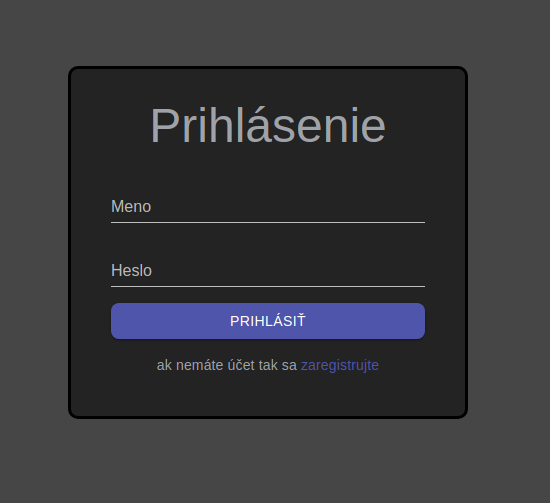
\includegraphics[width=0.8\textwidth]{images/prihlasenie}
  \caption[Prihlásenie]{Prihlásenie}
  \label{obr:prihlasenie}
\end{subfigure}%
\begin{subfigure}{.5\textwidth}
  \centering
  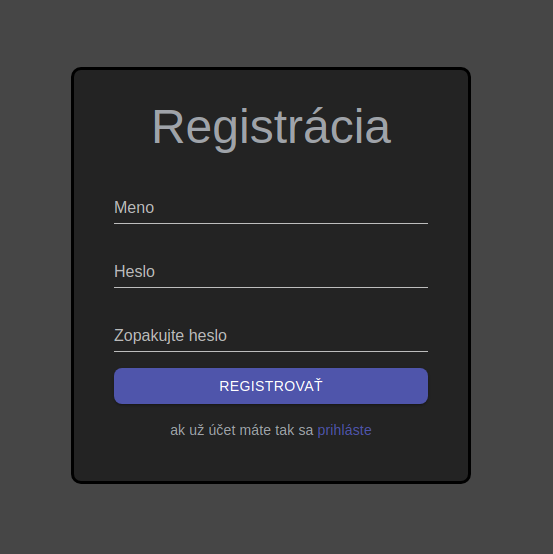
\includegraphics[width=0.8\textwidth]{images/registracia}
  \caption[Registrácia]{Registrácia}
  \label{obr:registracia}
\end{subfigure}
\caption{Prihlásenie a registrácia}
\end{figure}

Prihlasovací formulár validuje, či je používateľ zaregistrovaný a či zadal správne heslo. Podobne
registrovací formulár kontroluje, či je používateľské meno voľne a či sa heslá zhodujú. Prípadné
chyby zobrazuje pod formulárom.
\begin{figure}[H]
\centering
\begin{subfigure}{.5\textwidth}
  \centering
  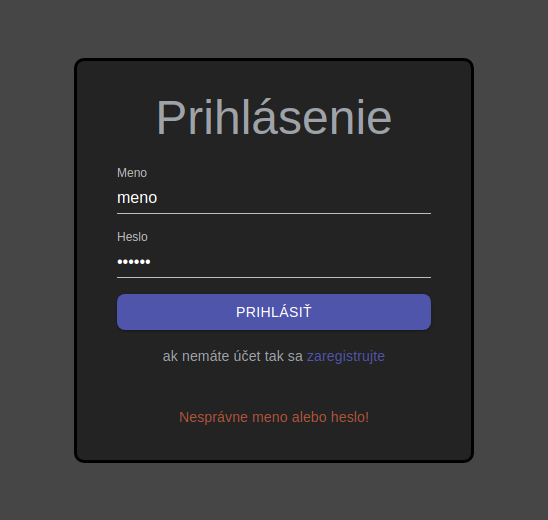
\includegraphics[width=0.8\textwidth]{images/validacia_prihlasenie}
  \caption[Validácia prihlásenia]{Validácia prihlásenia}
  \label{obr:validacia_prihlasenie}
\end{subfigure}%
\begin{subfigure}{.5\textwidth}
  \centering
  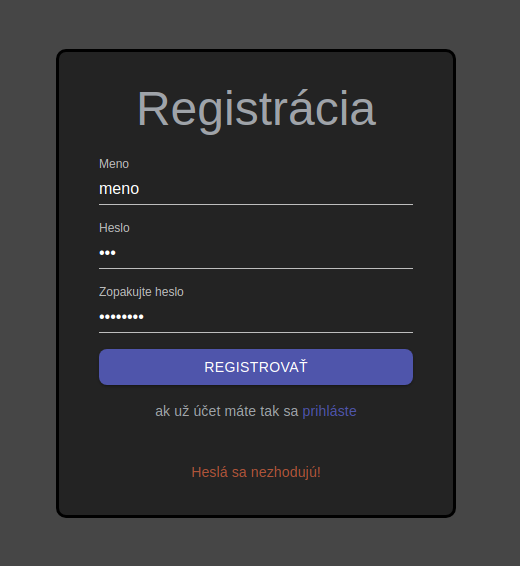
\includegraphics[width=0.8\textwidth]{images/validacia_registracia}
  \caption[Validácia registrácie]{Validácia registrácie}
  \label{obr:validacia_registracia}
\end{subfigure}
\caption{Validácia prihlásenia a registrácie}
\end{figure}

Po prihlásení používateľa sa zobrazí hlavná časť programu. Odlišuje sa však výrazne podľa toho, či
je prihlásený používateľ administrátor alebo bežný používateľ.

\subsection{Rozhranie pre bežného používateľa}
Po prihlásení sa zobrazí bežnému používateľovi rozhranie, v ktorom vidí všetky vytvorené skupiny.
Nevidí však ani ich obsah ani prihlásených pouźívateľov patriacich do daných skupín. Do skupín
ho vie pridať iba administrátor. Ďalej śu v rozhraní zobrazené skupiny, do ktorých používateľ patrí
a v nich vidí aj ostatných pouźívateľov spolu so zadaniami pre danú skupinu.
% TODO: obrazok ked (ak) to bude implementovane

Ak si používateľ vybral zadanie, otvorí sa mu editor, v ktorom vie upravovať všetky súbory dostupné
pre dané zadanie. Súčasťou editora sú viaceré komponenty, ktoré používateľovi uľahčujú a
zprehľadňujú prácu s editorom. 
\begin{figure}[H]
\centerline{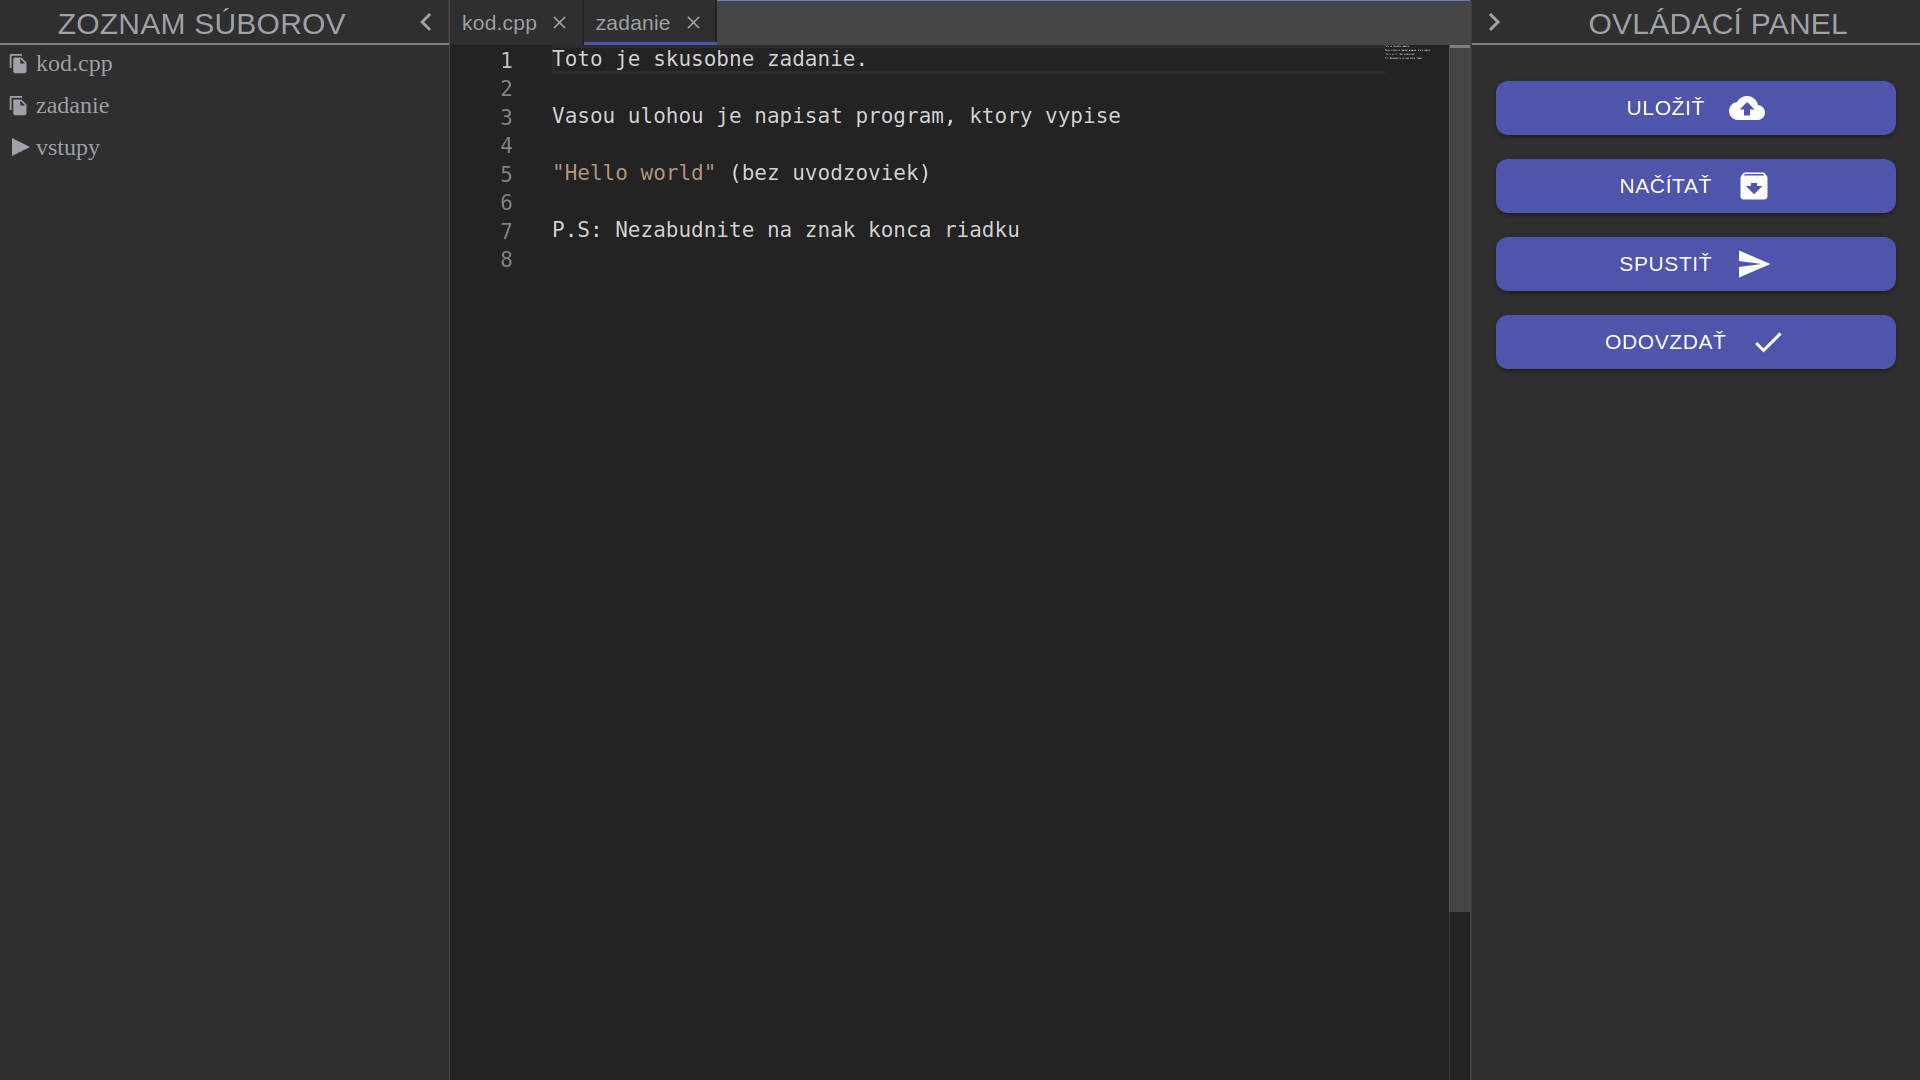
\includegraphics[width=1\textwidth]{images/bezny_pouzivatel}}
\caption[Editor zadania]{Editor zadania}
\label{obr:bezny_pouzivatel}
\end{figure}

% https://tex.stackexchange.com/questions/5035/paragraph-style-how-to-force-line-break-paragraph-make-paragraph-a-he
\paragraph{Panel so zoznamom súborov}\leavevmode\\
Komponent, ktorý obsahuje hierarchickú schému priečinkov a súborov dostupných v zadaní. Priečinky sa
dajú otvárať podobne ako pri otváraní súboru na počítači. Súbor alebo priečinok, na ktorý ukazuje
kurzor sa zvýrazňuje a kurzor sa zmení na ukazateľ aby užívateľ vedel, že môže na danú vec kliknúť.
Ikonky jasne odlišujú súbor a priečinok. Priečinok môže byť v schovanom alebo zobrazenom stave. 
Tieto stavy sú rozlíšené typom ikonky.
\begin{figure}[H]
\centering
\begin{subfigure}{.5\textwidth}
  \centering
  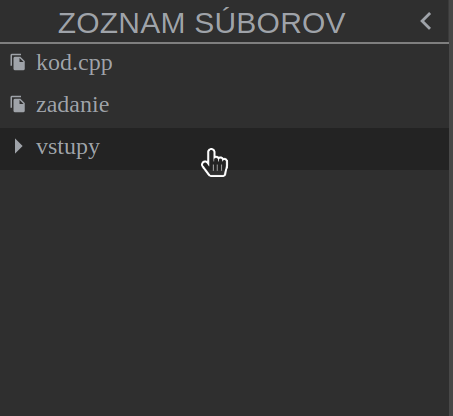
\includegraphics[width=0.8\textwidth]{images/schovany_zoznam}
  \caption[Schovaný obsah priečinka]{Schovaný obsah priečinka}
  \label{obr:schovany_zoznam}
\end{subfigure}%
\begin{subfigure}{.5\textwidth}
  \centering
  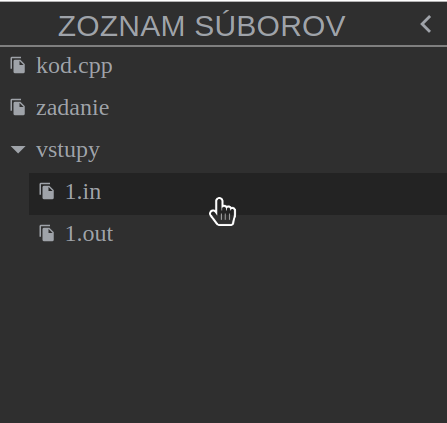
\includegraphics[width=0.8\textwidth]{images/zobrazeny_zoznam}
  \caption[Zobrazný obsah priečinka]{Zobrazný obsah priečinka}
  \label{obr:zobrazeny_zoznam}
\end{subfigure}
\caption{Priečinok v zozname súborov}
\end{figure}

% https://tex.stackexchange.com/questions/5035/paragraph-style-how-to-force-line-break-paragraph-make-paragraph-a-he
\paragraph{Ovládací panel}\leavevmode\\
Ovládací panel umožňuje používateľovi vykonávať akcie so svojím zadaním. Používateľ si môže svoj kód
uložiť, načítať, spustiť na vlastnom vstupe a otestovať na skrytých vstupoch tak ako to bolo 
napísané v návhu. Pri kliknutí na ľubovolnú akciu sa zobrazí dialóg, v ktorom používateľ doplní
ďalšie údaje a potvrdí akciu, ktorá sa následne vykoná na serveri.

Pri ukladaní zadania je nutné zvoliť identifikátor, pod ktorým sa má zadanie uložiť. Identifikátor
môže obsahovať iba písmená anglickej abecedy, čísla a pomlčku. Ak užívaťel zadá neplatný 
identifikátor, klient mu súbor uložiť nedovolí.
\begin{figure}[H]
\centering
\begin{subfigure}{.5\textwidth}
  \centering
  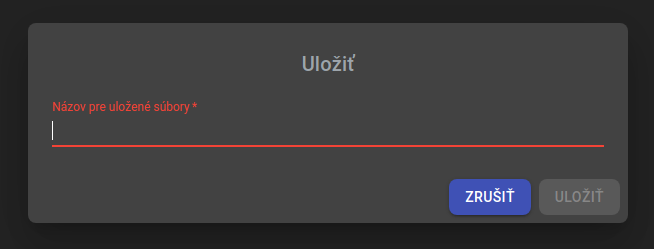
\includegraphics[width=0.8\textwidth]{images/neplatny_nazov}
  \caption[Neplatný názov identifikátora]{Neplatný názov identifikátora}
  \label{obr:neplatny_nazov}
\end{subfigure}%
\begin{subfigure}{.5\textwidth}
  \centering
  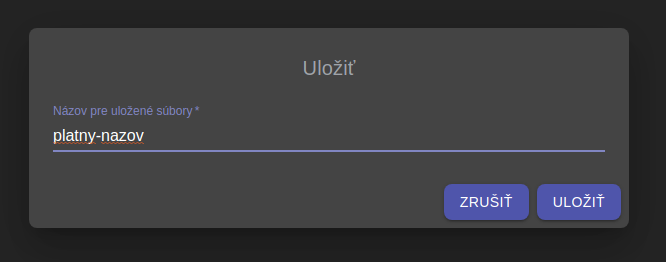
\includegraphics[width=0.8\textwidth]{images/platny_nazov}
  \caption[Platný názov identifikátora]{Platný názov identifikátora}
  \label{obr:platny_nazov}
\end{subfigure}
\caption{Uloženie zadania}
\end{figure}

Pri načítavaní uloženého zadania sa užívateľovi zobrazia všetky jemu dostupné uložené zadania v 
zozname. Používateľ si vie vybrať ktorý záznam chce načítať poďla identifikátora, ktorý zadával
pri ukladaní a časovej pečiatky, kedy záznam uložil. Okrem iného, aplikácia niekedy robí ukladanie
sama od seba. Používateľ si vie povedať, či chce takéto záznamy vidieť v možnostiach.
\begin{figure}[H]
\centering
\begin{subfigure}{.5\textwidth}
  \centering
  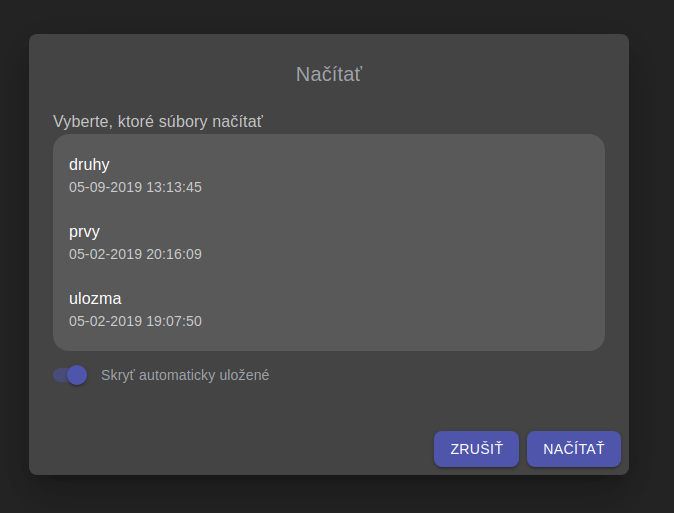
\includegraphics[width=0.8\textwidth]{images/nacitaj_zadanie}
  \caption[Iba vlastné uloženia]{Iba vlastné uloženia}
  \label{obr:nacitaj_zadanie}
\end{subfigure}%
\begin{subfigure}{.5\textwidth}
  \centering
  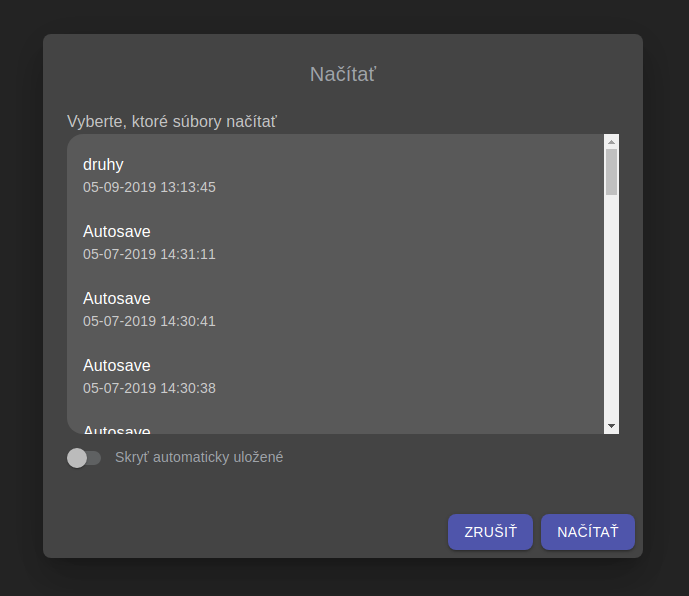
\includegraphics[width=0.8\textwidth]{images/nacitaj_automaticky_ulozene}
  \caption[Zobrazené aj automaticky uložené]{Zobrazené aj automaticky uložené}
  \label{obr:platny_nazov}
\end{subfigure}
\caption{Načítanie zadania}
\end{figure}

Po kliknutí na spustiť sa zobrazí dialóg, v ktorom vie používateľ zadať vlastný vstup a následne 
spustiť svoj program na danom vstupe. Užívateľ potom v dialógu potvrdí spustenie a program sa spolu
so vstupom ktorý zadal odošle na server, kde sa momentálny stav zadania automaticky uloží,
skompiluje a následne spustí. Počas behu programu sa v dialógu zmení tlačítko, ktoré upozorňuje, že
program beží. Po skončení behu programu sa zobrazí výsledný výstup v dialógu.
\begin{figure}[H]
\centering
\begin{subfigure}{.3\textwidth}
  \centering
  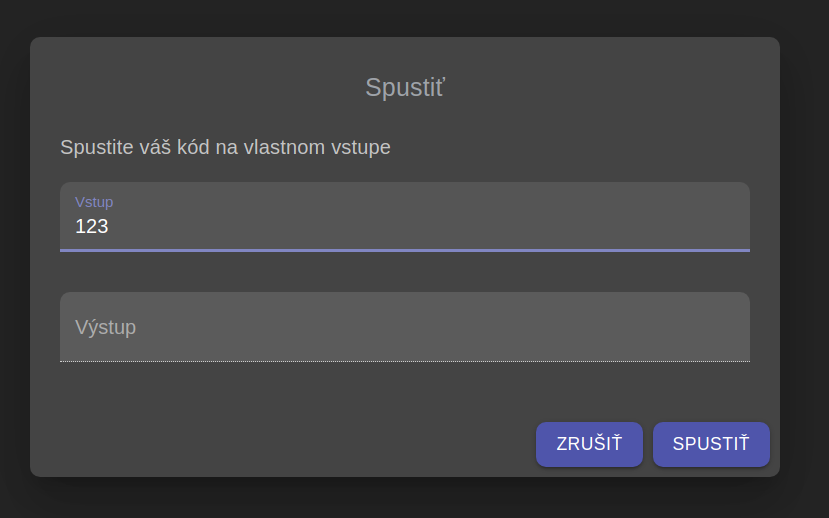
\includegraphics[width=0.9\textwidth]{images/spusti_dialog}
  \caption[Pred spustením]{Pred spustením}
  \label{obr:spusti_dialog}
\end{subfigure}%
\begin{subfigure}{.3\textwidth}
  \centering
  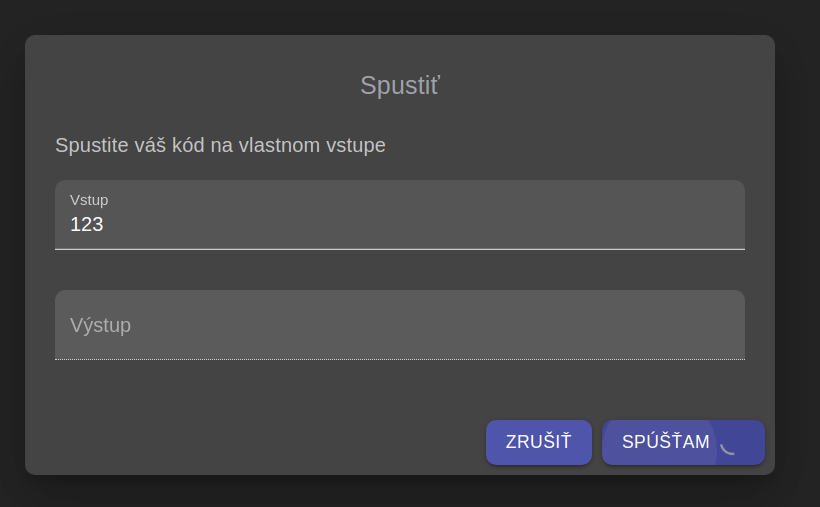
\includegraphics[width=0.9\textwidth]{images/spusti_dialog_beh}
  \caption[Počas behu]{Počas behu}
  \label{obr:spusti_dialog_beh}
\end{subfigure}
\begin{subfigure}{.3\textwidth}
  \centering
  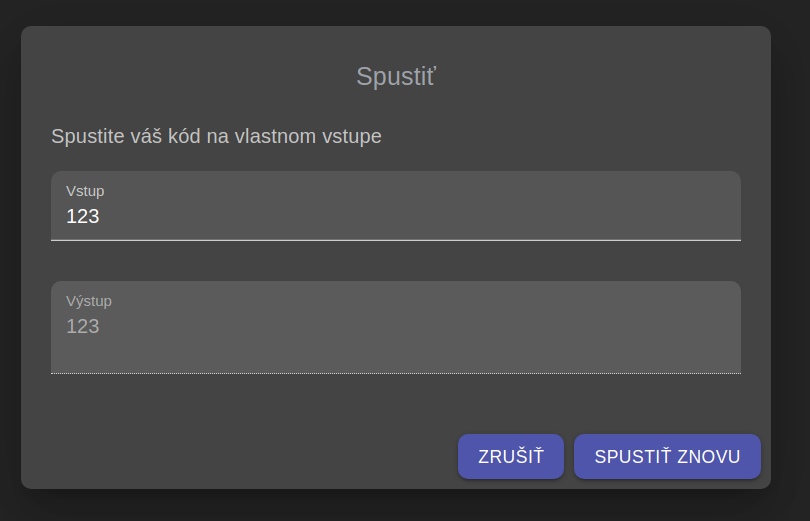
\includegraphics[width=0.9\textwidth]{images/spusti_dialog_koniec}
  \caption[Po dokončení]{Po dokončení}
  \label{obr:spusti_dialog_koniec}
\end{subfigure}
\caption{Spúštanie na vlastnom vstupe}
\end{figure}

Posledná akcia, ktorú vie používateľ spraviť je otestovanie svojho riešenia na skrytých vstupoch
uložených na serveri. Po kliknutí na tlačítko sa odošle na server aktuálny stav zadania, ktorý sa
na serveri uloží a automaticky začne testovať.
\begin{figure}[H]
\centering
\begin{subfigure}{.5\textwidth}
  \centering
  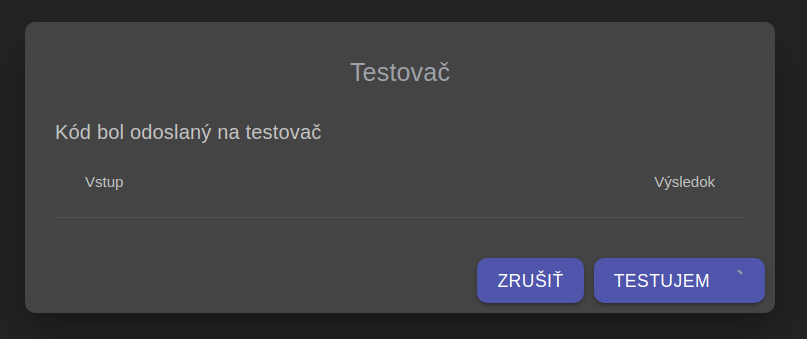
\includegraphics[width=0.8\textwidth]{images/testovanie_priebeh}
  \caption[Dialóg počas testovania]{Dialóg počas testovania}
  \label{obr:testovanie_priebeh}
\end{subfigure}%
\begin{subfigure}{.5\textwidth}
  \centering
  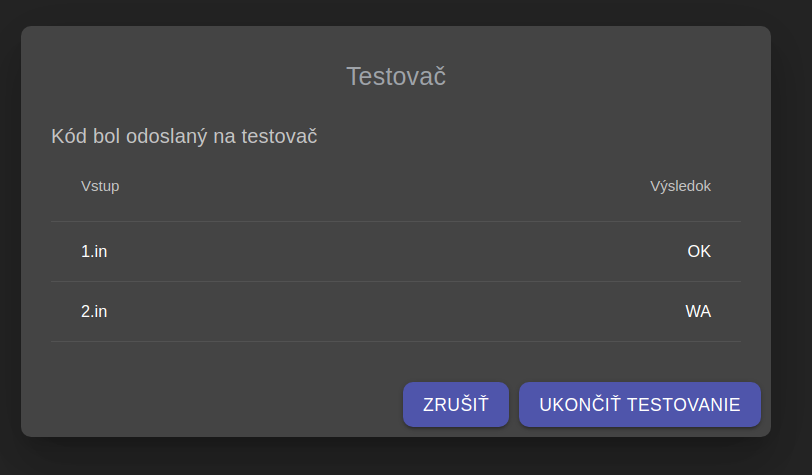
\includegraphics[width=0.8\textwidth]{images/testovanie_koniec}
  \caption[Dialóg po skončení testovania]{Dialóg po skončení testovania}
  \label{obr:testovanie_koniec}
\end{subfigure}
\caption{Testovanie na skrytých vstupoch}
\end{figure}

% https://tex.stackexchange.com/questions/5035/paragraph-style-how-to-force-line-break-paragraph-make-paragraph-a-he
\paragraph{Schované panely}\leavevmode\\
Oba panely zaberajú značný horizontálny priestor a nie vždy sú pre používateľa nutné. Má teda
možnosť panly schovať. Priestor, ktorý vznikne schovaním panelov vyplní editor. Používateľ môže
kedykoľvek panel zobraziť naspať kliknutím na šípku, ktorá panel vyroluje a editor sa zmenší. 
\begin{figure}[H]
\centerline{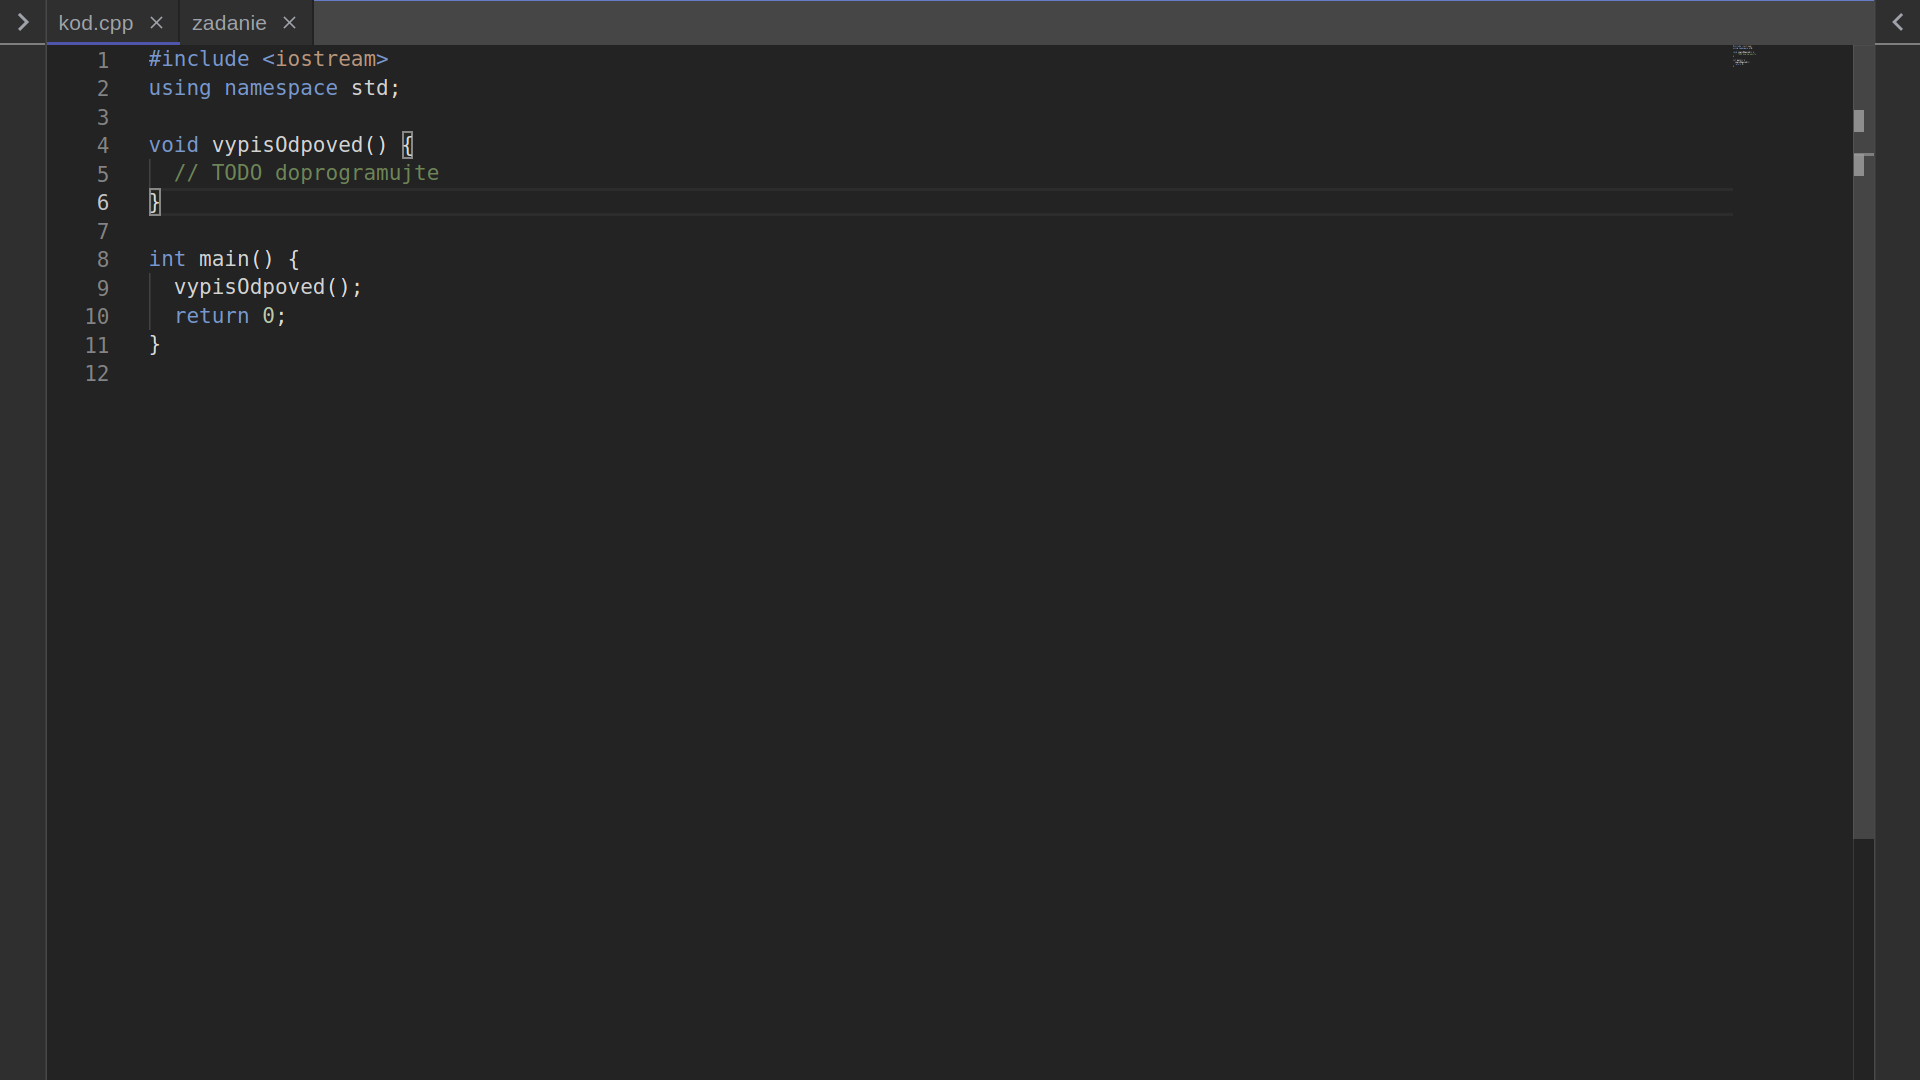
\includegraphics[width=1\textwidth]{images/zcucnute_panely}}
\caption[Editor zadania]{Editor zadania}
\label{obr:zcucnute_panely}
\end{figure}

\subsection{Rozhranie pre administrátora}
% TODO:

\section{Server}
% TODO:

\section{Izolované spúštanie kódu na serveri}
\label{kap:isolated_env} % id kapitoly pre prikaz ref

Kód spustený na serveri, nesmie narušiť ostatné programy, prípadne inak narušiť prostredie servera.
